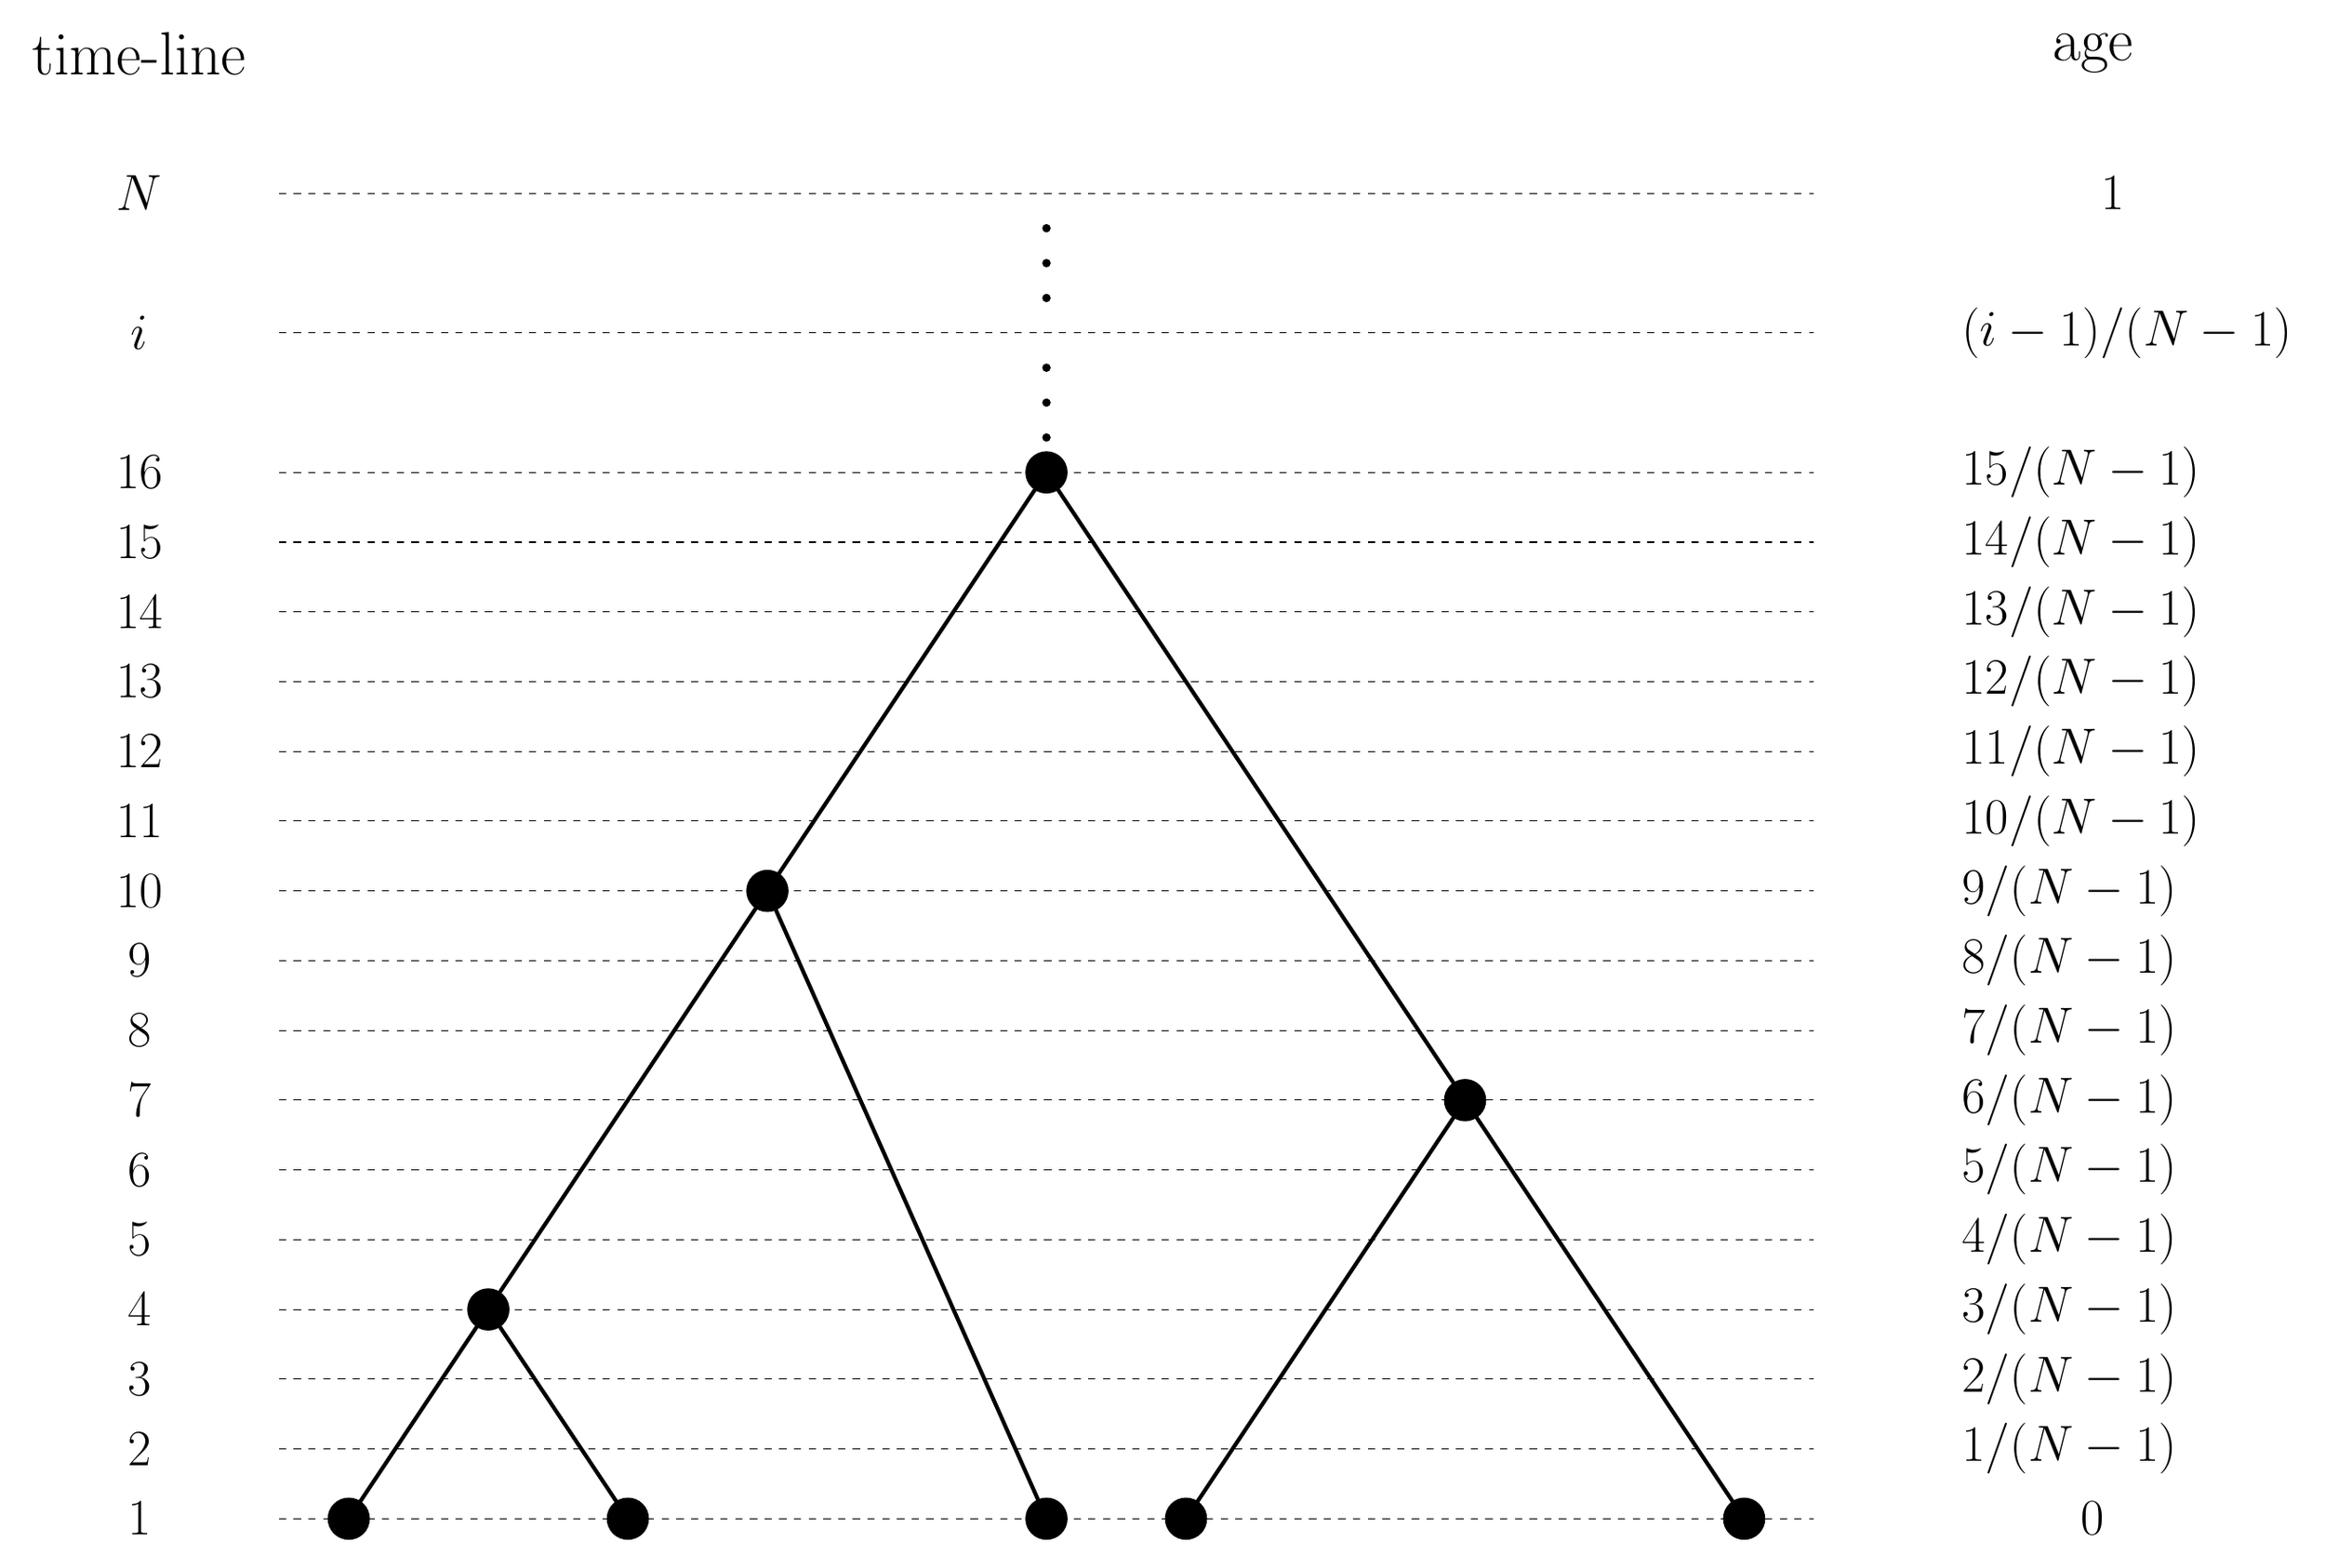
\begin{tikzpicture}[font=\Huge]
%\draw[step=1,gray,very thin] (0,0) grid (22,18);

\coordinate (a) at (11,16);

\coordinate (a1) at (11,1);
\coordinate (a2) at (1,1);

\coordinate (t1) at (3,4);
\fill (t1) circle (2ex);
\coordinate (t2) at (5,1);
\fill (t2) circle (2ex);
\draw[ultra thick] [-] (t1) -- (t2);

\fill (a) circle (2ex);
\fill (a1) circle (2ex);
\fill (a2) circle (2ex);

\draw[ultra thick] [-] (a) -- (a2);

\coordinate (b) at (7,10);
\fill (b) circle (2ex);
\draw[ultra thick] [-] (b) -- (a1);


\coordinate (a4) at (17,7);
\fill (a4) circle (2ex);

\coordinate (a5) at (13,1);
\fill (a5) circle (2ex);
\draw[ultra thick] [-] (a4) -- (a5);

\coordinate (a3) at (21,1);
\fill (a3) circle (2ex);
\draw[ultra thick] [-] (a) -- (a3);

% time-lines

\foreach \i in {1,...,16}
{
  \draw[dashed] [-] (0,\i) -- (22,\i);
}
  \draw[dashed] [-] (0,18) -- (22,18);
  \draw[dashed] [-] (0,20) -- (22,20);

% fill the ellipsis between time-line i

\fill (11,16.5) circle (0.4ex);
\fill (11,17) circle (0.4ex);
\fill (11,17.5) circle (0.4ex);


\fill (11,18.5) circle (0.4ex);
\fill (11,19) circle (0.4ex);
\fill (11,19.5) circle (0.4ex);

% time-line labels

\node at (-2,22) {time-line};
\foreach \i in {1,...,16}
{
  \node[font=\huge] at (-2,\i) {\i};
}

\node[font=\huge] at (-2,18) {$i$};

\node[font=\huge] at (-2,20) {$N$};

% ages

\node at (26,22) {age};

\node[font=\huge] at (26,1) {$0$};
\foreach \i in {1,...,15}
{
  \node[font=\huge,anchor=west] at (24,\i + 1) {$\i/(N-1)$};
}
\node[font=\huge,anchor=west] at (24,18) {$(i-1)/(N-1)$};
\node[font=\huge,anchor=west] at (26,20) {$1$};

\end{tikzpicture}
